% $Header: /home/vedranm/bitbucket/beamer/solutions/conference-talks/conference-ornate-20min.en.tex,v 90e850259b8b 2007/01/28 20:48:30 tantau $

\documentclass{beamer}


\mode<presentation>
{
  \usetheme{Warsaw}
  %\usetheme{default}
  % or ...

  \setbeamercovered{transparent}
  % or whatever (possibly just delete it)
}


\usepackage[english]{babel}
% or whatever

\usepackage[latin1]{inputenc}
% or whatever

\usepackage{times}
\usepackage[T1]{fontenc}
\usepackage{amsmath}
\usepackage{epstopdf}
\usepackage{multirow}
\usepackage{gensymb}
% Or whatever. Note that the encoding and the font should match. If T1
% does not look nice, try deleting the line with the fontenc.


\title[Recent results and discussions] % (optional, use only with long paper titles)
{Landauer Experiment \\Recent results and discussions 2}


%\author[Shreyas Bhaban]{Shreyas Bhaban}% (optional, use only with lots of authors)

\institute[U of M] % (optional, but mostly needed)
{
 Department of Electrical Engineering\\
 University of Minnesota\\
}
% - Use the \inst command only if there are several affiliations.
% - Keep it simple, no one is interested in your street address.

\date{\today}



\AtBeginSubsection[]
{
  \begin{frame}<beamer>{Outline}
    \tableofcontents[currentsection,currentsubsection]
  \end{frame}
}


\begin{document}

\begin{frame}
  \titlepage
\end{frame}

\begin{frame}{Outline}
  \tableofcontents  % You might wish to add the option [pausesections]
\end{frame}

%%-----------------------------------------------------------------------------------------------------------------


%%-----------------------------------------------------------------------
\section{Understanding approach in the Nature paper}
\begin{frame}{What has been done in Nature paper-1} 

\begin{figure}
    \centering
    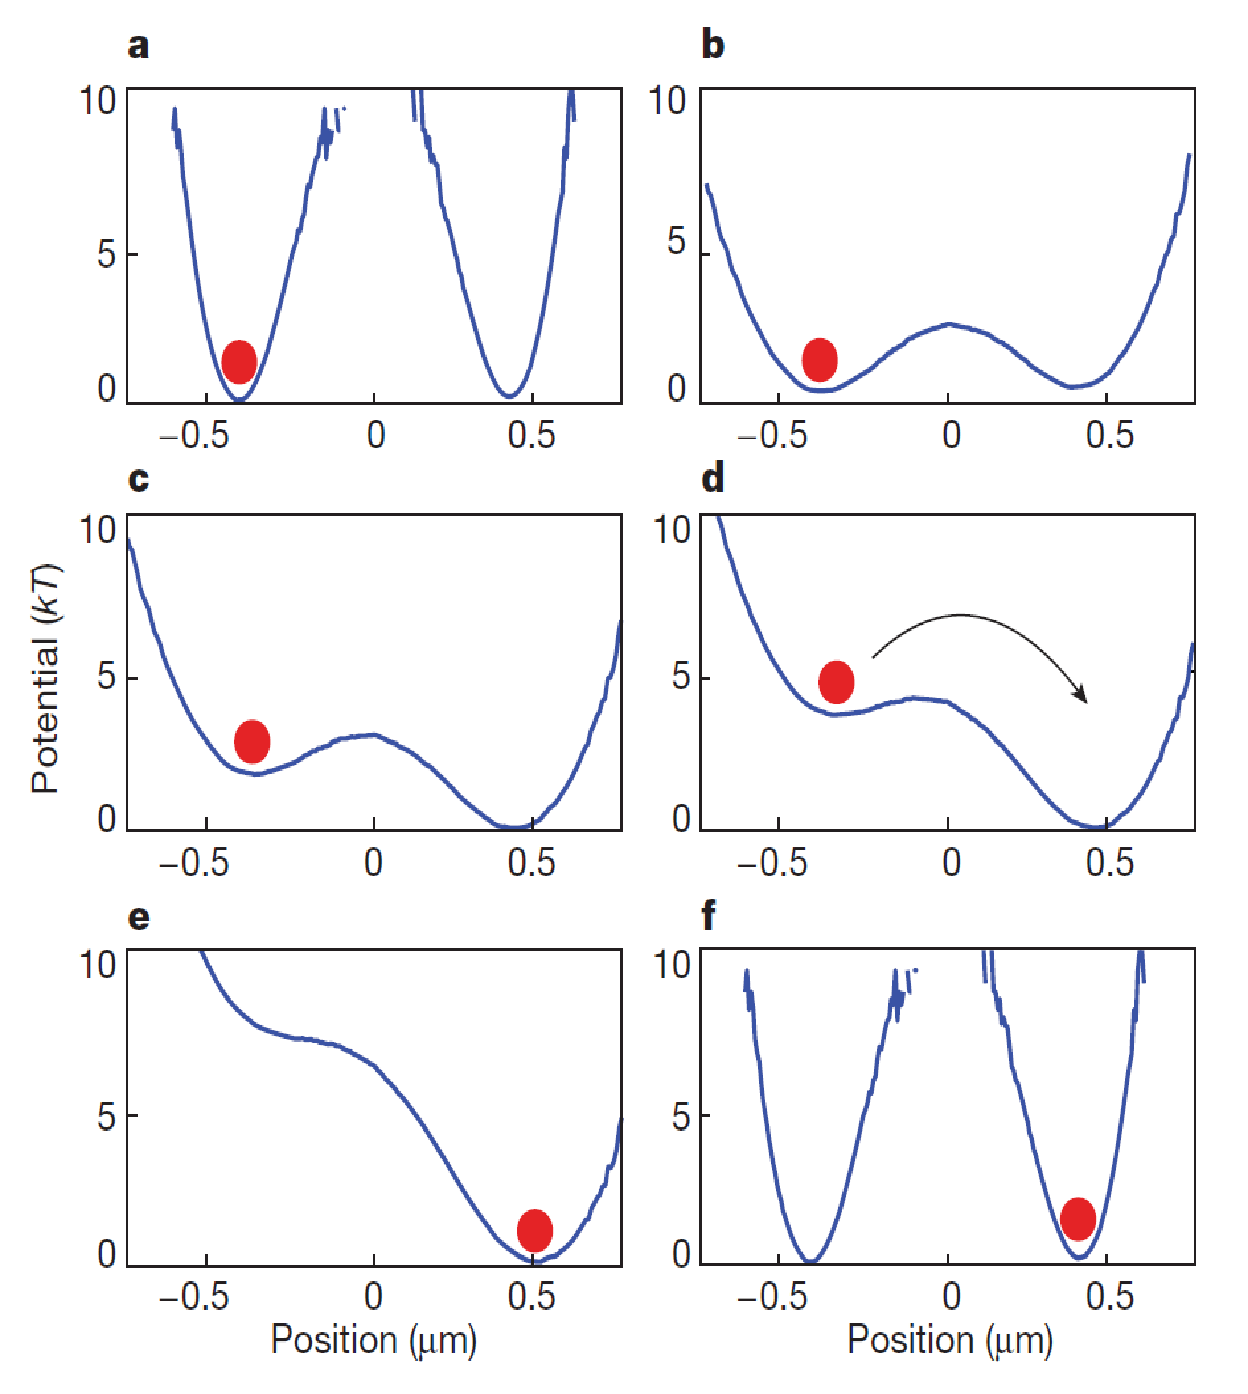
\includegraphics[height=5cm,width=11cm]{nature_landauer_fig1.eps}
 %   \caption{Applying step fitting to bead trace}
    \label{fig:graph26}
\end{figure}

\end{frame}
%%-----------------------------------------------------------------------
\begin{frame}{What has been done in Nature paper-2} 

For fig. a,b and f the plots are found using experimental data as:
\begin{itemize}

\item Well potential calculated using pdf is used via.
\begin{equation*}
U_0(x,I_L) = -K_BT~ln[(P(x,I_L)]
\end{equation*}
\item According to paper, the measured $U_0(x,I_L)$ is plotted in fig.a,b,f and can be fitted by $8^{th}$ order polynomial as :
\begin{equation*}
U_0(x,I_L) = \sum_{n=0}^8 u_n(I_L,d_f)x^n
\end{equation*}
where $d_f$ is the distance between the two points over which laser is switched ($1450~nm$ here)

\end{itemize}

\end{frame}
%%-----------------------------------------------------------------------
\begin{frame}{What has been done in Nature paper-3} 

For fig. c,d and e the plots are found using following calculations :
\begin{itemize}

\item Total time of erasure = Time of stage motion with increasing velocity = $\tau$
\item Amplitude of viscous force is increased linearly during time $\tau$ : $F(t)=\pm F_{max}t/\tau$
\item Intermediate plots during transfer is calculated at three different values of time $t$ :
\begin{equation*}
U(x,t) = U_0(x,I_L)- F_{max}(t/\tau).x
\end{equation*}
\item \textit{I suspect, the plot in fig.b is also an $8^{th}$ order fit, since the contours in the plots from b to e are the same}

\end{itemize}

\end{frame}
%%-----------------------------------------------------------------------
\begin{frame}{Our approach-1} 

Points of discussion last time :
\begin{itemize}

\item How did they obtain good curve for saddle points ?
\item Their is not only a polynomial fit, but involves calculation using the $8^{th}$ order fitted curve $U_0(x,I_L)$ as :
\begin{equation*}
U(x,t) = U_0(x,I_L)- F(t)
\end{equation*}
\item This is why they obtain such good curve at the saddle point
\end{itemize}
Our approach to match their plots :
\begin{itemize}

\item Obtain fig. a and f using the photodiode data as they have done
\item Obtain the fig. d \textbf{which is the exact point of transfer} using actual data and fitted curve

\end{itemize}

\end{frame}
%%-----------------------------------------------------------------------
\begin{frame}{Our approach-2} 

\textbf{Replicated fig.a and f} with R=3.2 $K_BT$, SD = 48.3 nm, L = 3.4 $K_BT$, SD = 37.1 nm 
\begin{figure}
    \centering
    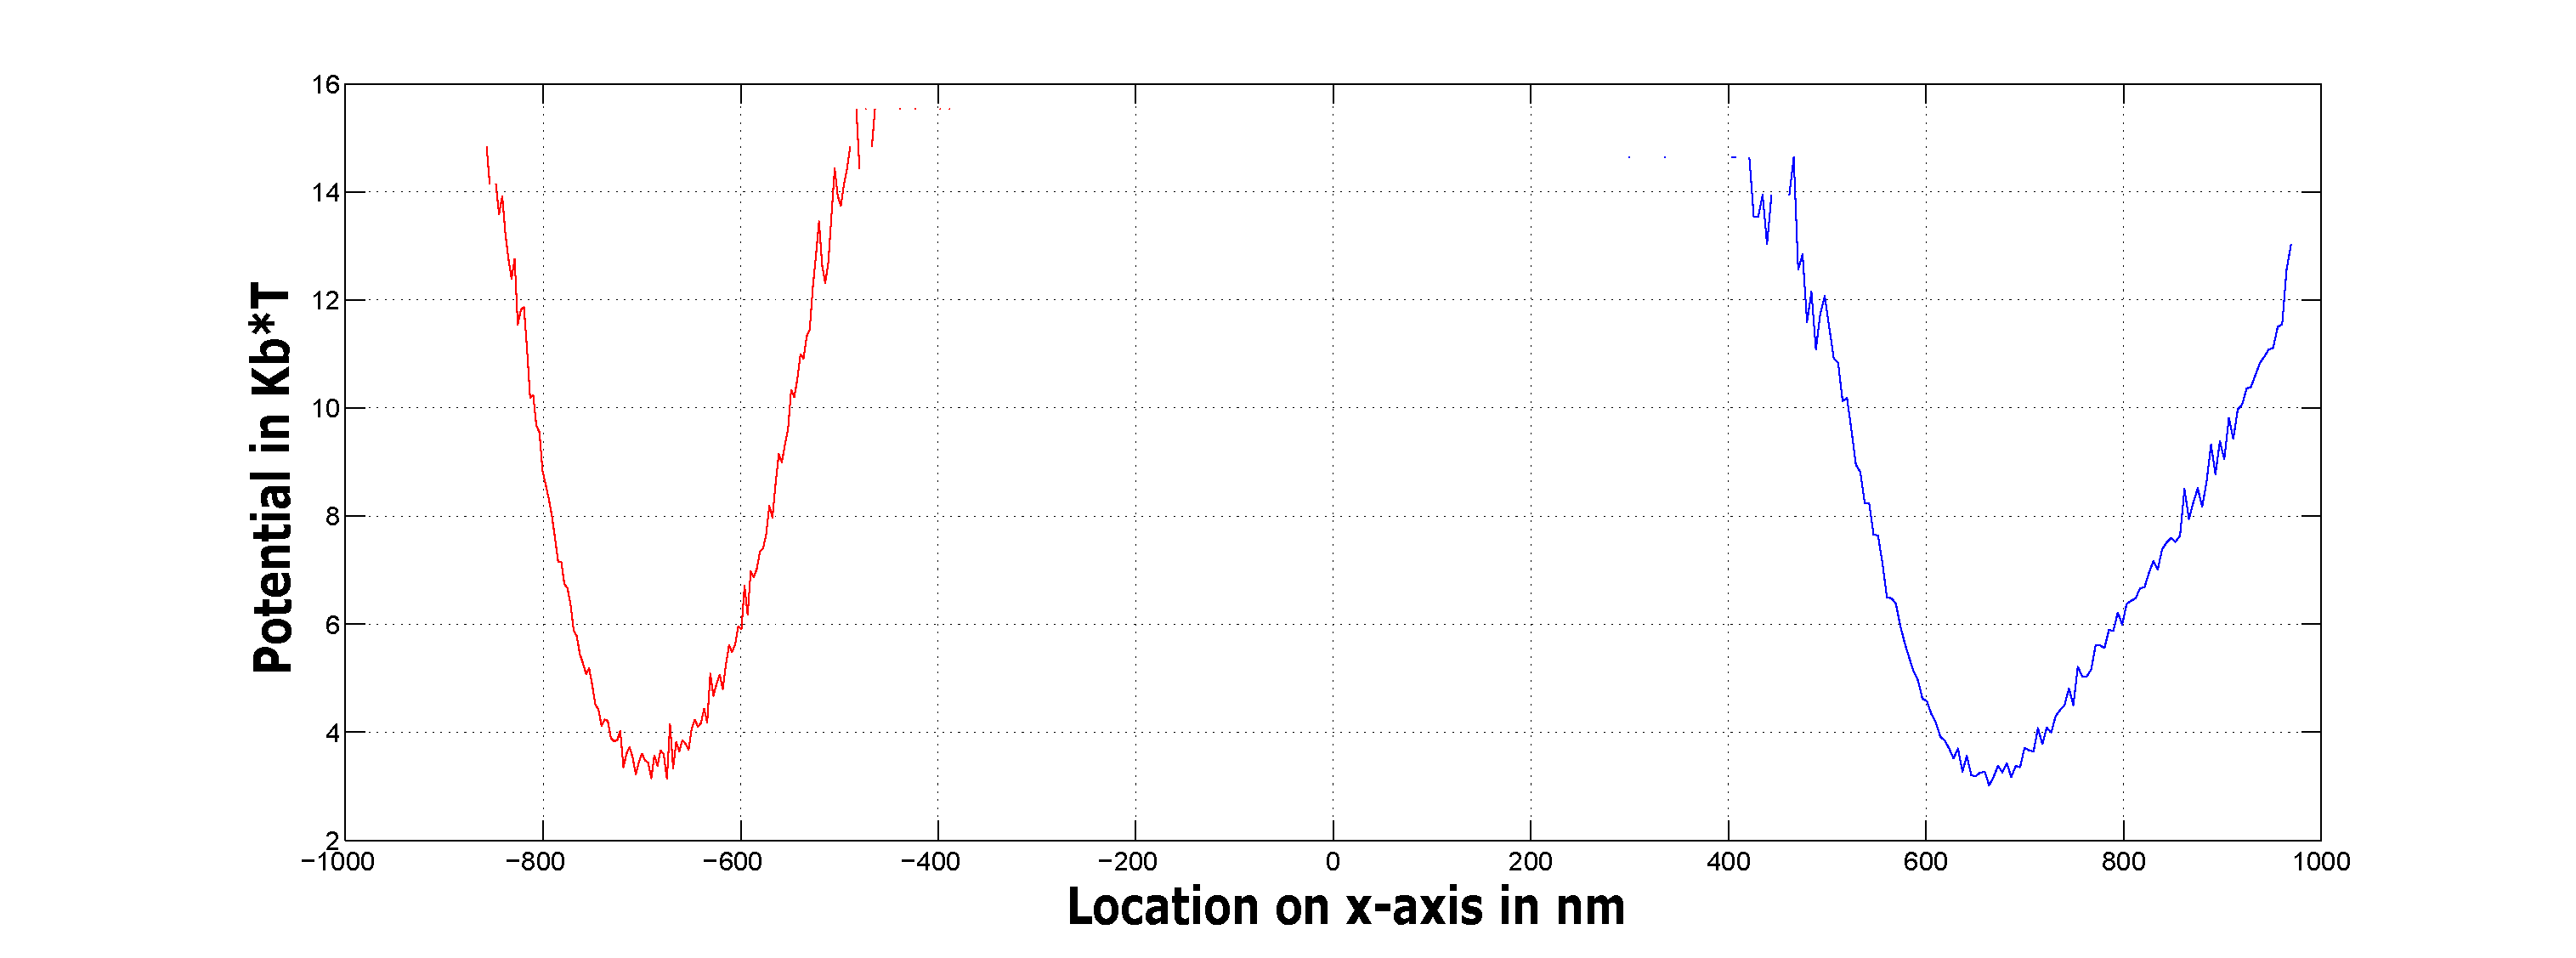
\includegraphics[height=4.5cm,width=12cm]{I4k_both_wells_700_1.eps}
 %   \caption{Applying step fitting to bead trace}

\end{figure}


\end{frame}


%%-----------------------------------------------------------------------
\begin{frame}{Our approach-3} 

\textbf{Replicated fig.d} \textit{at exact point of transfer} with blinks L=7 ,R=1 ; L = 2 $K_BT$,R = 3.3 $K_BT$, Height = 12.5 $K_BT$
\begin{figure}
    \centering
    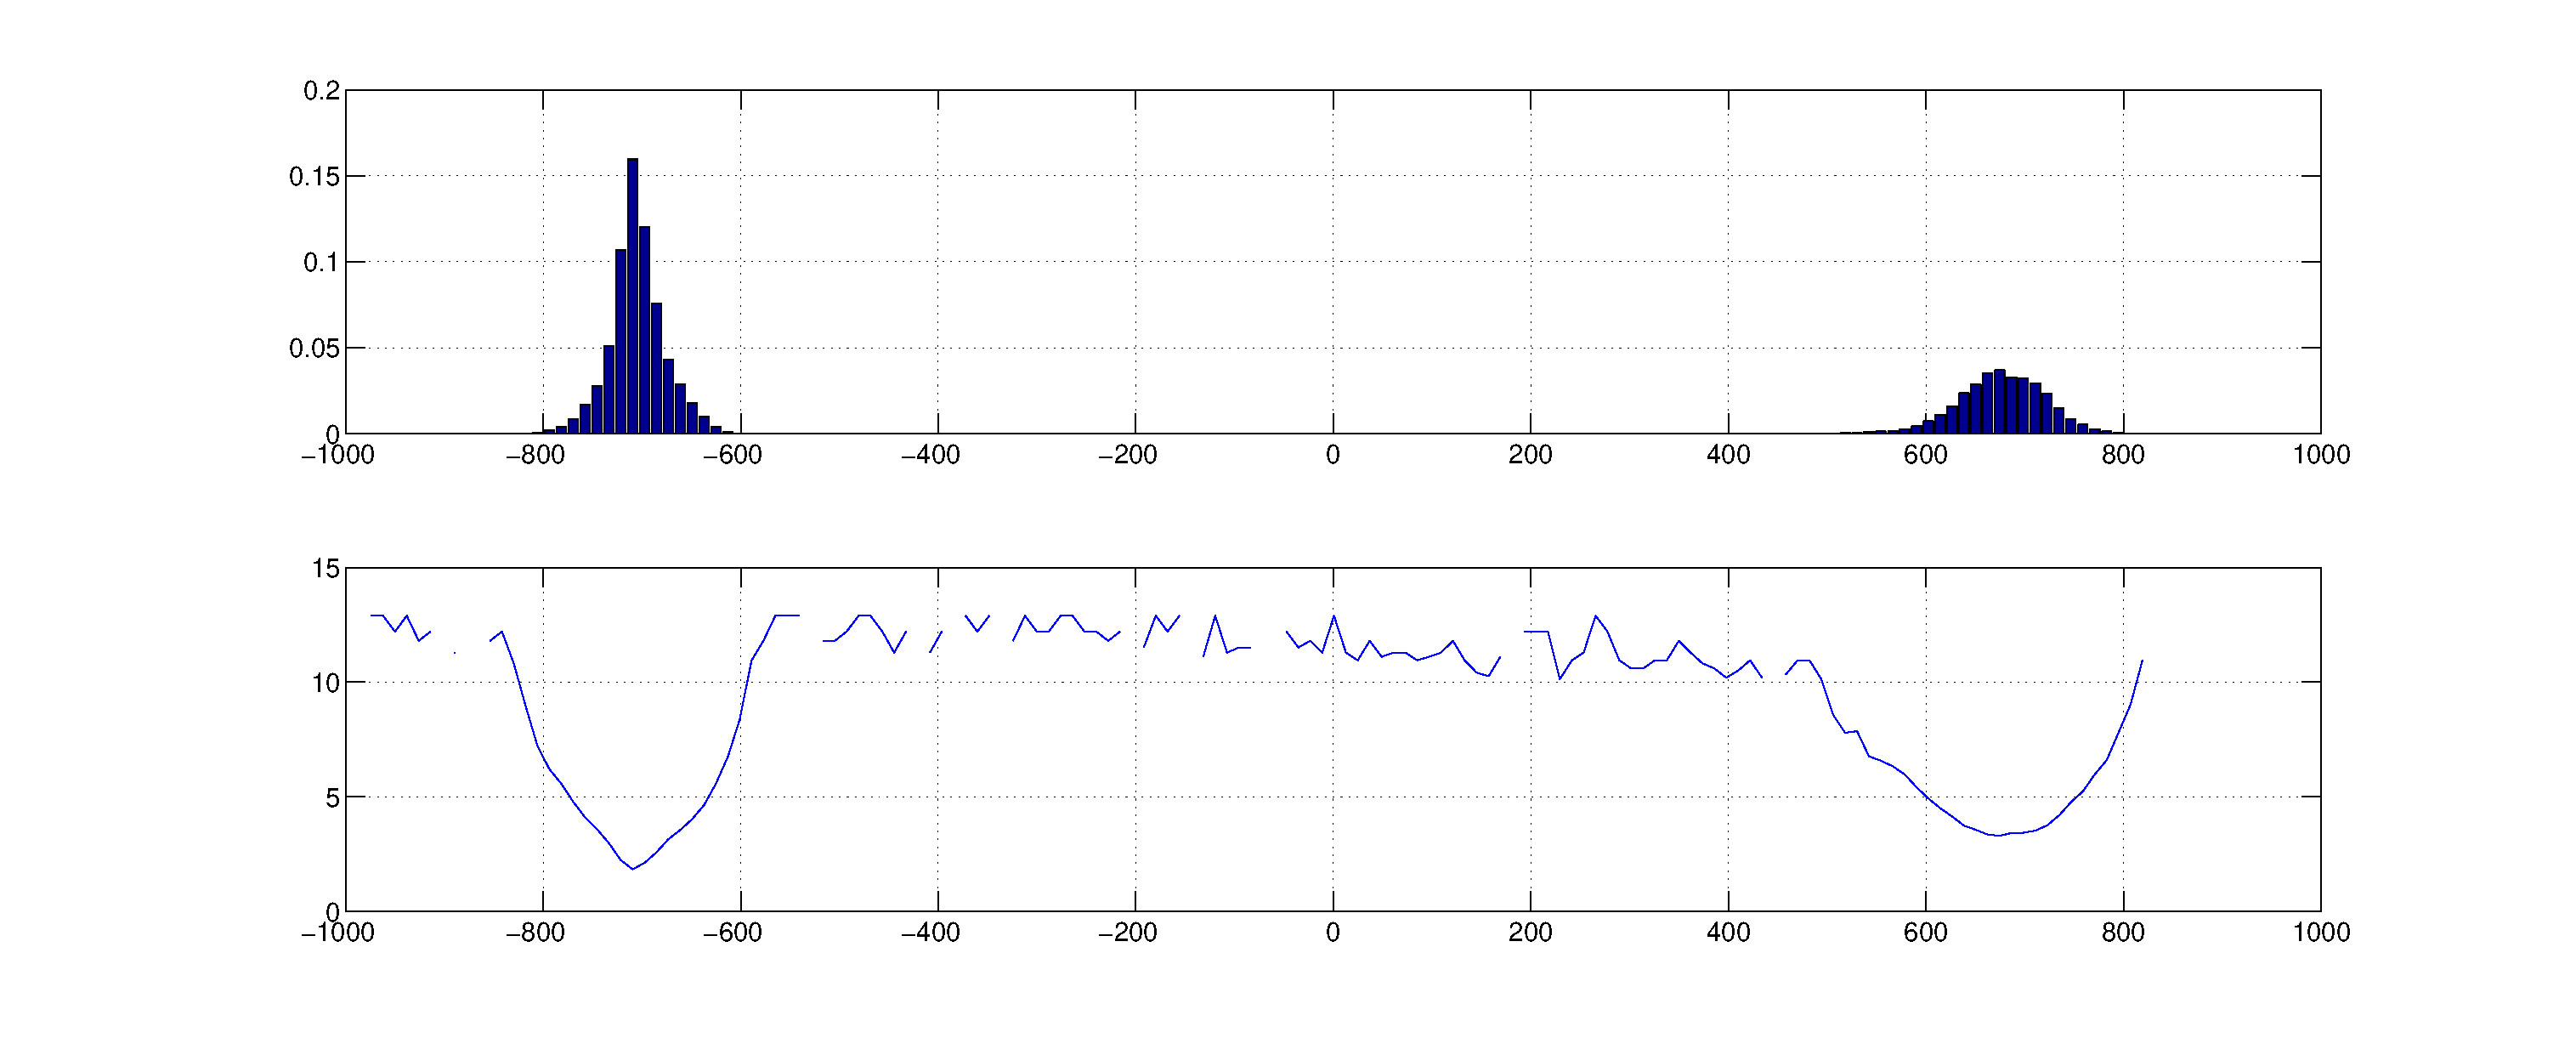
\includegraphics[height=5cm,width=12cm]{I4k_transfer_wells_6.eps}
 %   \caption{Applying step fitting to bead trace}
   
\end{figure}


\end{frame}


%%-----------------------------------------------------------------------
\begin{frame}{Our approach-4} 

To obtain good curve at saddle points, following is done :
\begin{itemize}

\item Several datasets depicting the exact points of transfer are obtained
\item Each individual potential well calculated using pdf is used via.
\begin{equation*}
U_0(x,I_L) = -K_BT~ln[(P(x,I_L)]
\end{equation*}
\item Several datasets averaged to depict actual wells
\item Polynomial fitted for comparison

\end{itemize}

\end{frame}

%%-----------------------------------------------------------------------
\begin{frame}{Outline}
  \tableofcontents  % You might wish to add the option [pausesections]
\end{frame}
%%-----------------------------------------------------------------------
\section{Tilting wells - Multiple transfers}
\begin{frame}{Multiple Transfers - Several examples} 

\begin{itemize}

\item Trap bead at +700; potential well formed at +700
\item Total 12 blinks fixed : for equal potential, 6 blinks for each well, each blink for 20 $\mu s$
\item R$\rightarrow$L transition seen from 8,4 onwards i.e. 8,4...9,3...10,2 and 11,1
\item To see the minimum tilt needed for this transition, 8,4 is fixed
\item Modulate the on times as :

\begin{center} 
\begin{tabular}{| l | c | r |} 
\hline Total & Left & Right \\ 
\hline 12 & 6 & 6 \\ 
\hline 12 & 7 & 5 \\ 
\hline 12 & 8 & 4 \\ 
\hline \hline 12 & 6 & 6 \\ 
\hline \end{tabular} 
\end{center}

\end{itemize}

\end{frame}

%%-----------------------------------------------------------------------
\begin{frame}{Averaging 7 instances of R$\rightarrow$L transfer at 8,4 blinks} 

\begin{figure}
    \centering
    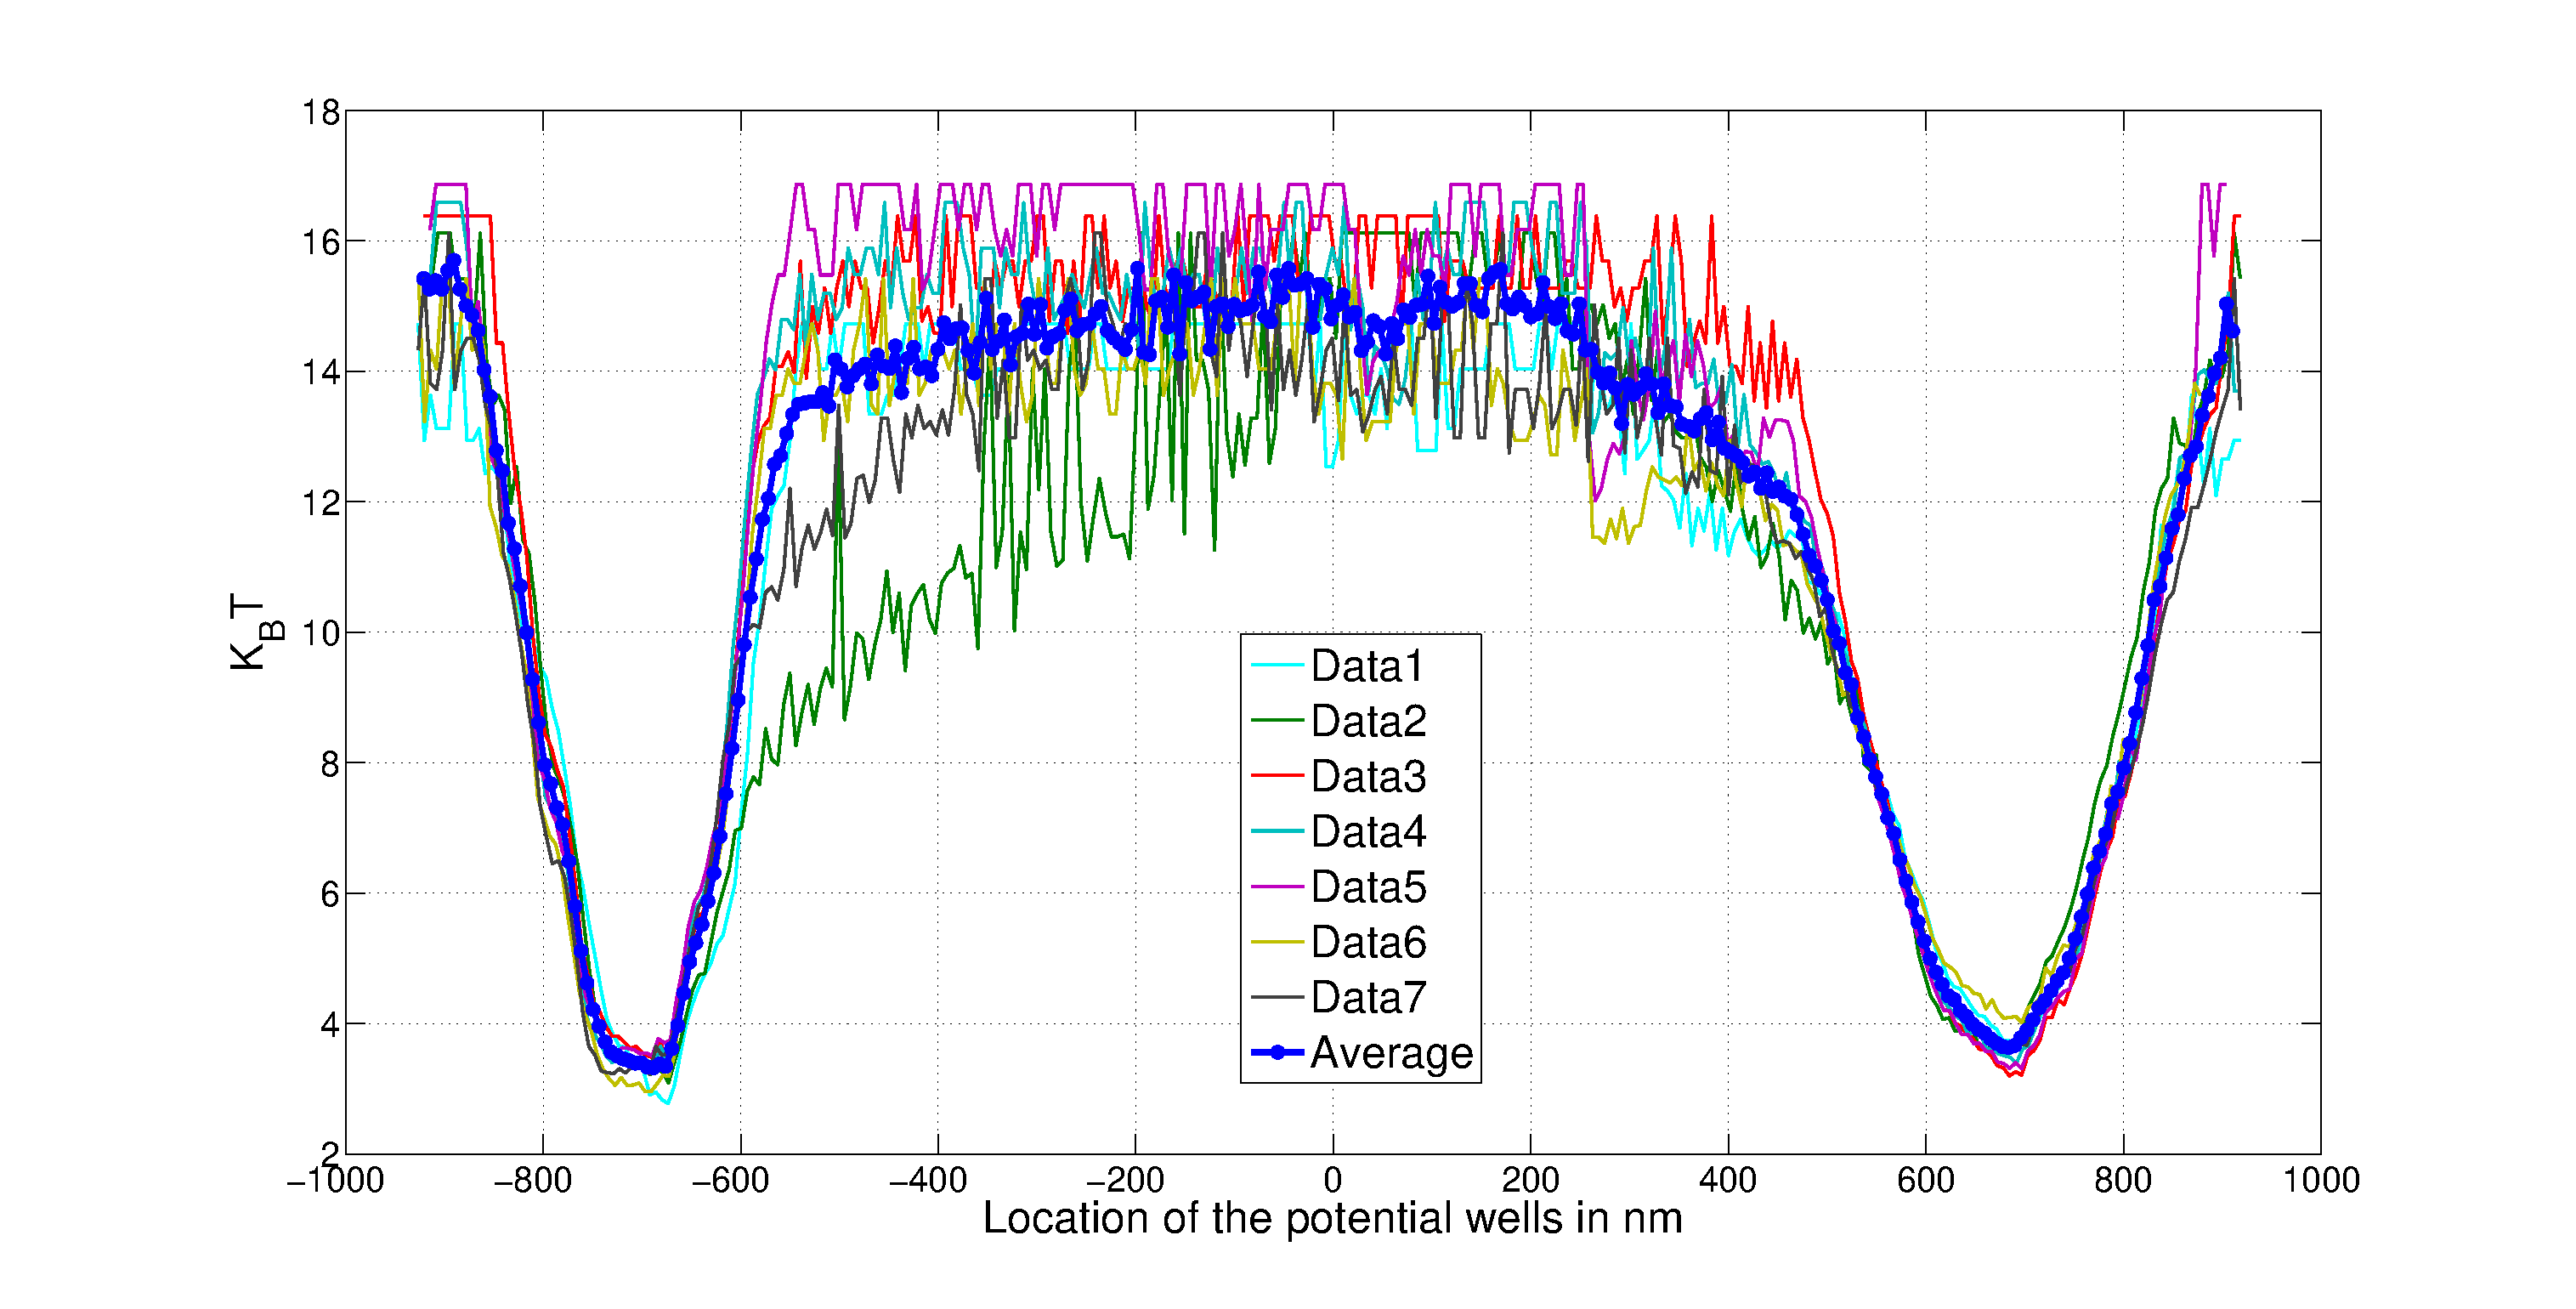
\includegraphics[height=6.5cm,width=12cm]{Mean_of_the_seven_potential_wells_probb1.eps}
 %   \caption{Applying step fitting to bead trace}
    \label{fig:graph27}
\end{figure}

\end{frame}
%%-----------------------------------------------------------------------
\begin{frame}{Polynomial fit- 8 th order, both wells together} 

\begin{figure}
    \centering
    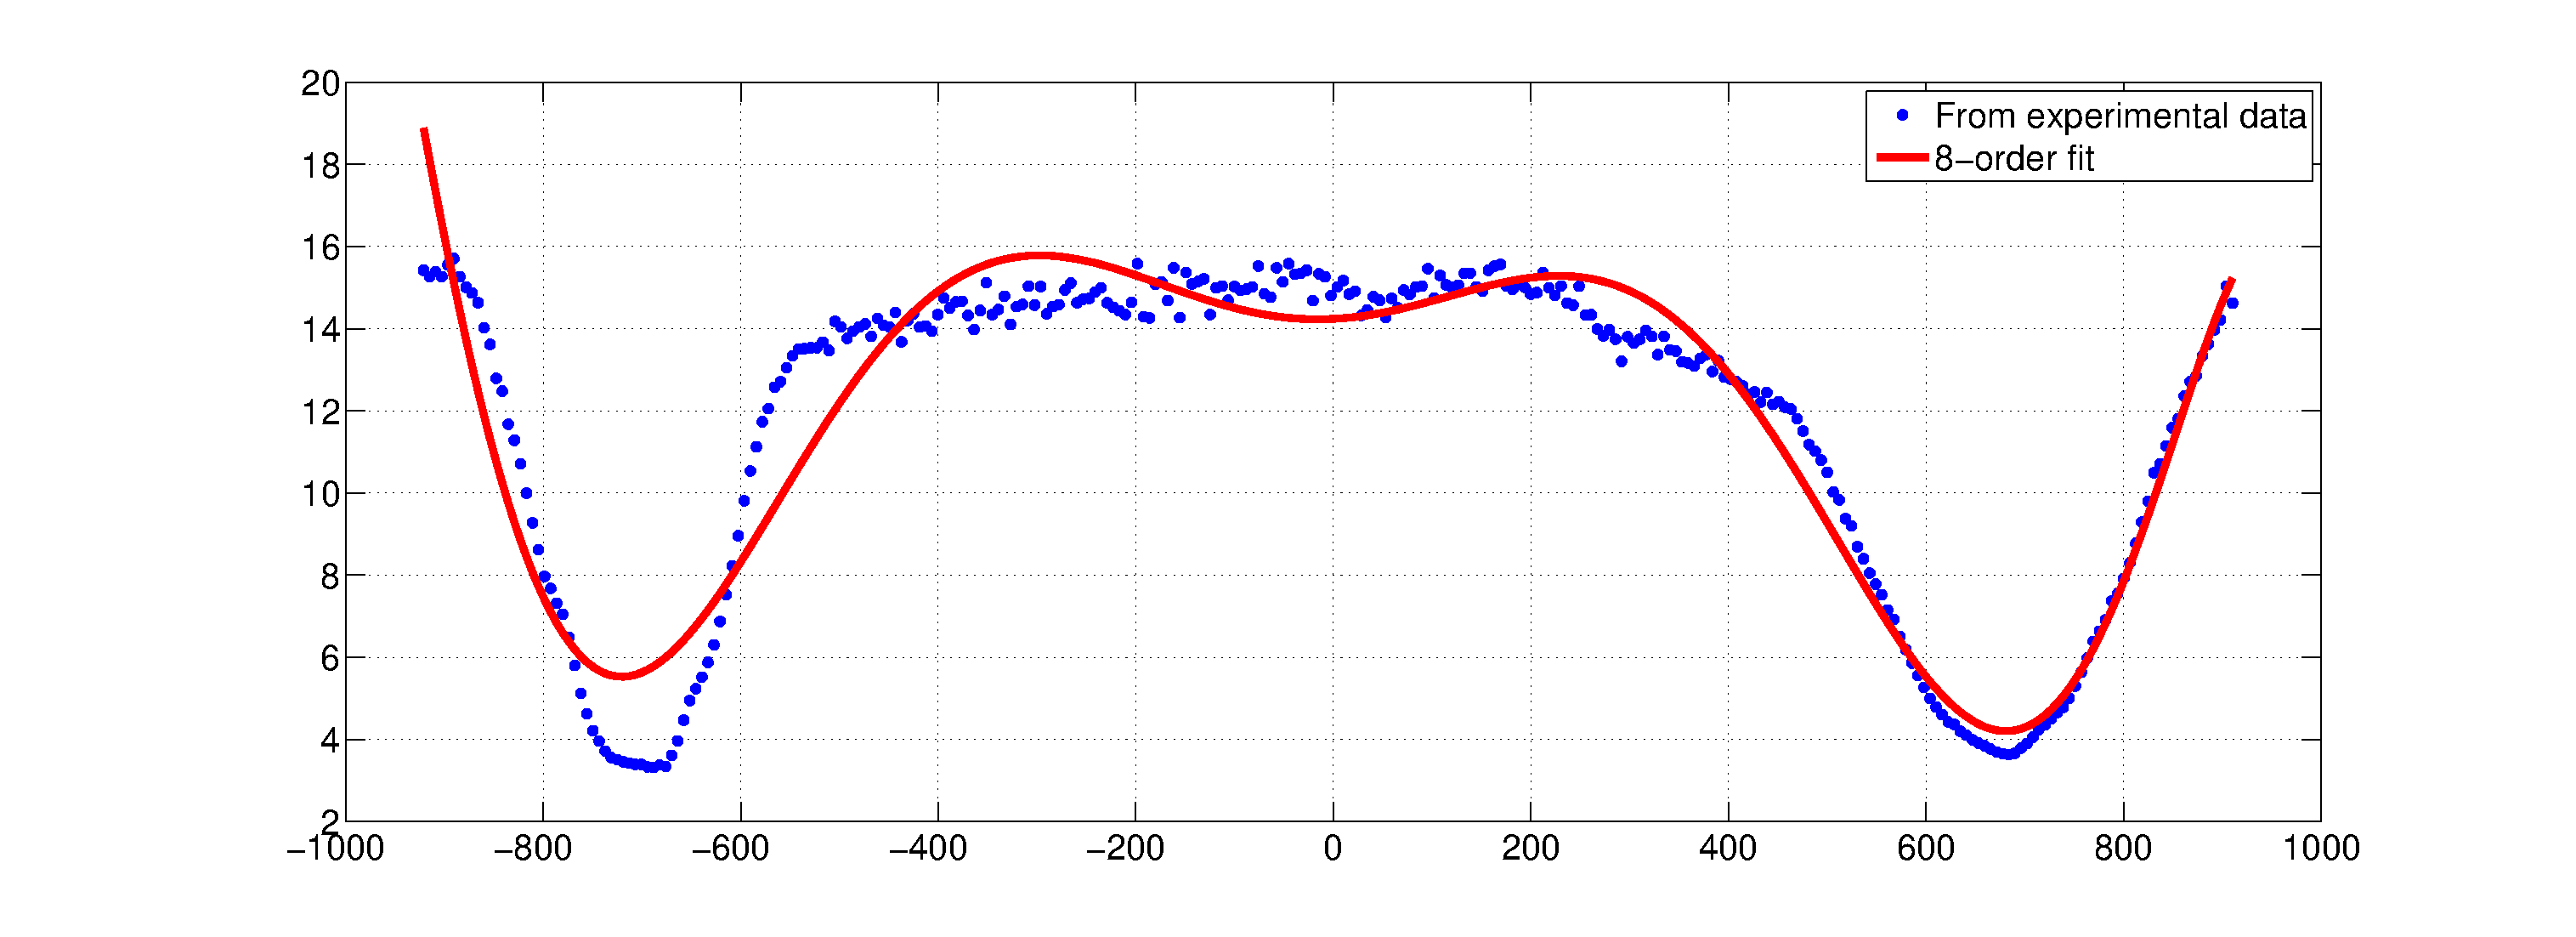
\includegraphics[height=6cm,width=11cm]{total_polyfit_probb1_8order.eps}
 %   \caption{Applying step fitting to bead trace}
    \label{fig:graph28}
\end{figure}

\end{frame}
%%-----------------------------------------------------------------------
\begin{frame}{Polynomial fit- 8 th order,R and L separately} 

\begin{figure}
    \centering
    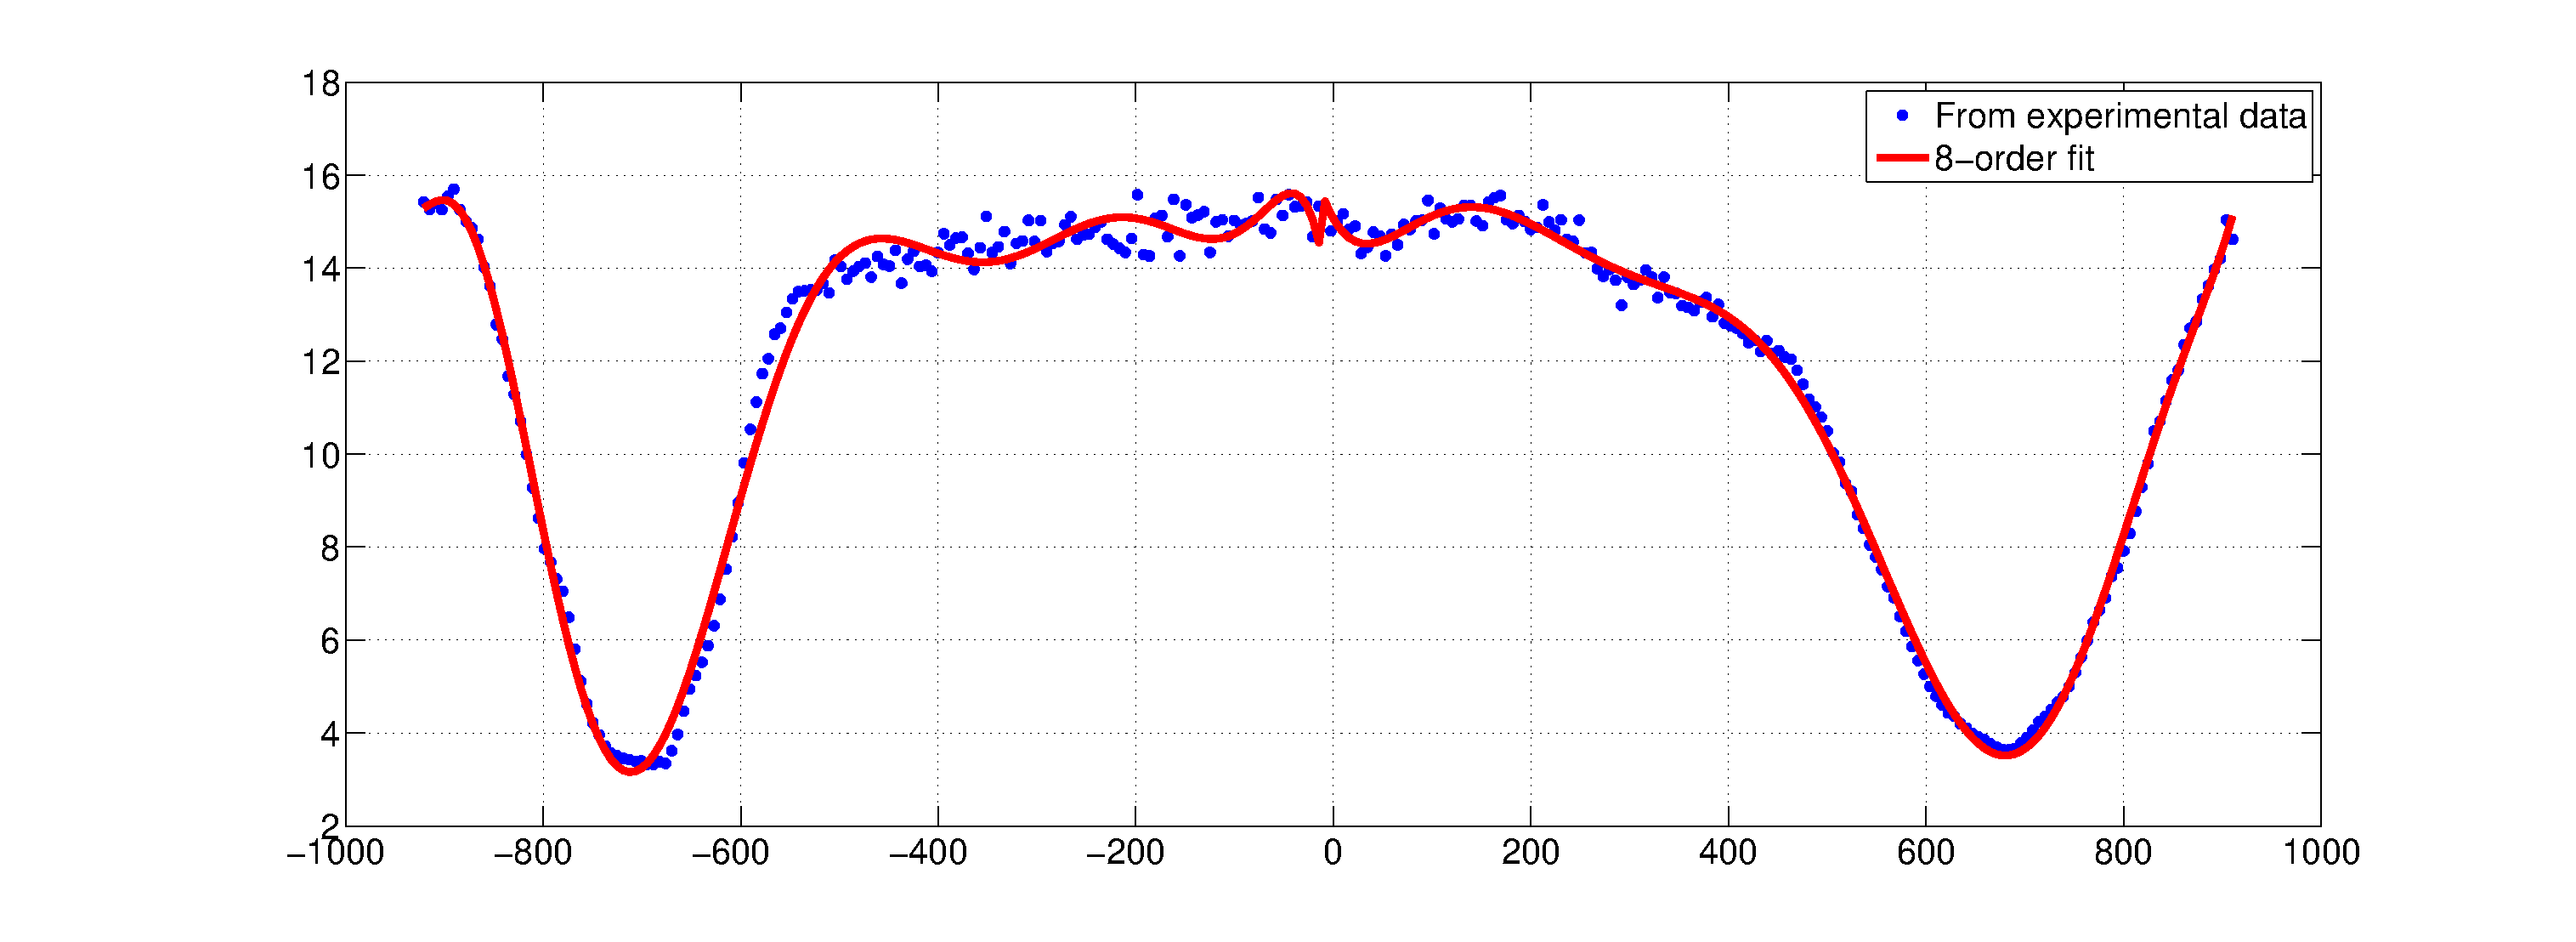
\includegraphics[height=6cm,width=11cm]{separate_polyfit_probb1_8order.eps}
 %   \caption{Applying step fitting to bead trace}
    \label{fig:graph29}
\end{figure}

\end{frame}

%%-----------------------------------------------------------------------
\begin{frame}{Polynomial fit- 15 th order,both wells together} 

\begin{figure}
    \centering
    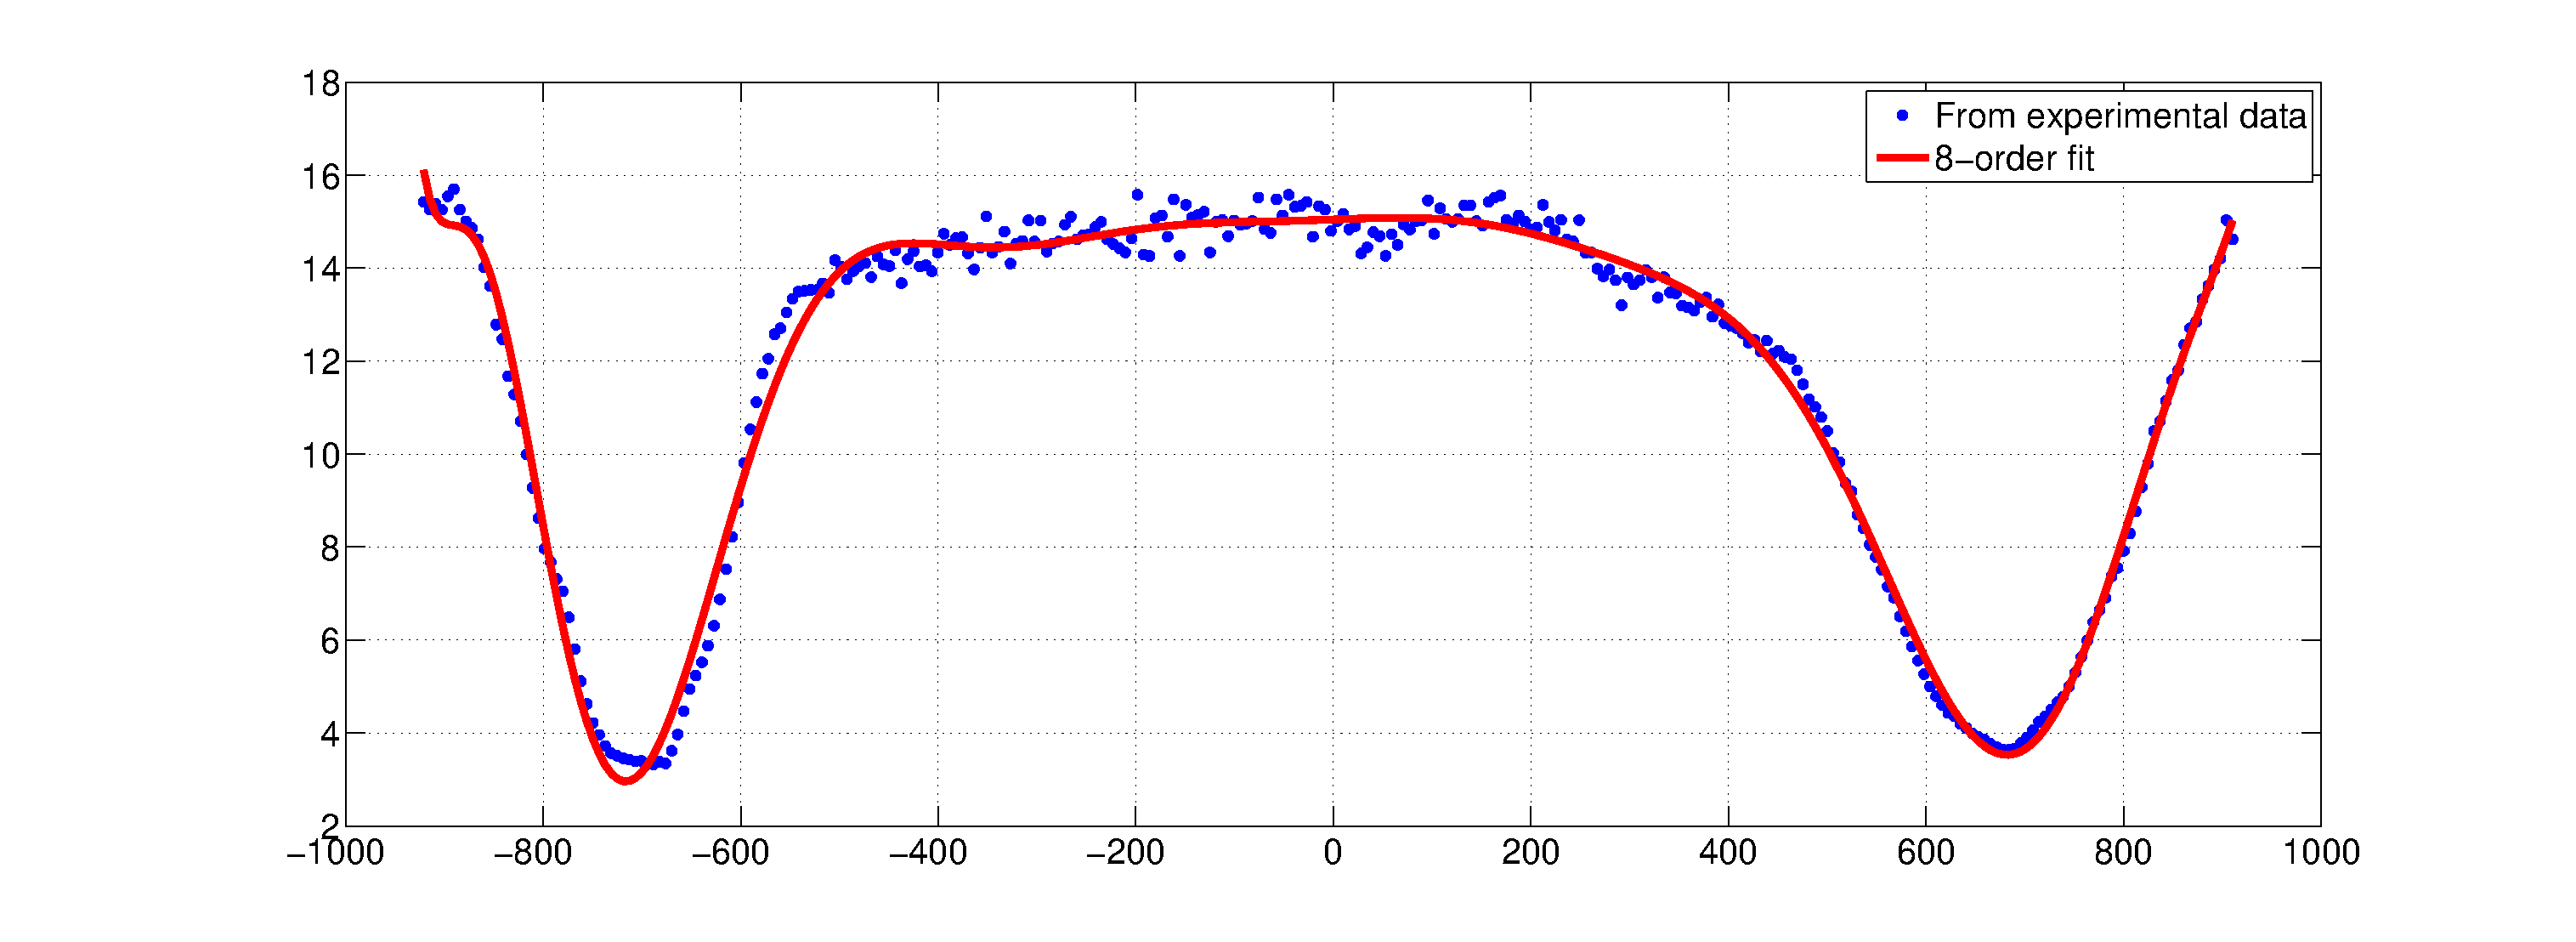
\includegraphics[height=6cm,width=11cm]{total_polyfit_probb1_15order.eps}
 %   \caption{Applying step fitting to bead trace}
    \label{fig:graph30}
\end{figure}

\end{frame}

%%-----------------------------------------------------------------------
\begin{frame}{Inference} 

\begin{itemize}

\item Averaging multiple transfers gives good graphical representation of the 'saddle point'
\item Fitting polynomial to both wells together needs higher order fit (at least $15^{th}$ order here)
\item Separately fitting R and L wells can be accomplished with lower order polynomials

\end{itemize}

\end{frame}

%%-----------------------------------------------------------------------
\begin{frame}{Outline}
  \tableofcontents  % You might wish to add the option [pausesections]
\end{frame}
%%-----------------------------------------------------------------------
\section{Work Done - Existing Literature}
\begin{frame}{Idea}

\textbf{Directly using calculated work done :}
\begin{itemize}

\item Calculate work done $W = \int_{t_1}^{t_2} F .dx$; Heat dissipated $Q = -\int_{t_1}^{t_2} F .dx$
\item $<Q>$ over several iterations should approach Landauer's limit $K_BT ln(2)$ 

\end{itemize} 

\textbf{Using Jarzynski's equality :}
\begin{itemize}

\item For a quasi-static process $<W> \approx \Delta F $
\item Using $<e^{-\beta W}> ~=~ e^{-\beta \Delta F}$, find $\Delta F$, the free energy difference
\item The value $\Delta F_{eff}=-ln(<e^{-\beta W}>)$ is always close to the Landauer's limit $K_BT ln(2)$, \textit{independent of the maximal force or procedure duration}$^*$

\end{itemize} 
\tiny{Detailed Jarzynski equality applied to logically irreversible procedure, A.Berut et al, EPL, 2013}
\end{frame}
%%-----------------------------------------------------------------------

\subsection{Work done in Nature Paper}
\begin{frame}{Work done in the Nature paper}

\begin{figure}
    \centering
    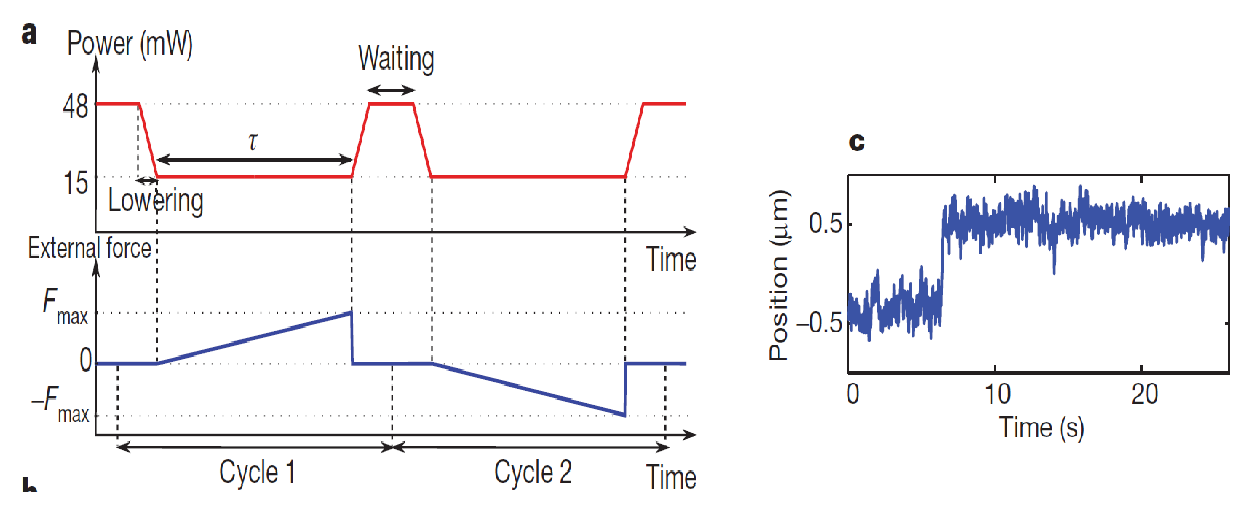
\includegraphics[height=5cm,width=11cm]{nature_landauer_fig2.eps}
 %   \caption{Applying step fitting to bead trace}
    \label{fig:graph2}
\end{figure}



\end{frame}

%%-----------------------------------------------------------------------
\begin{frame}{Work done in the Nature paper}
\begin{figure}
    \centering
    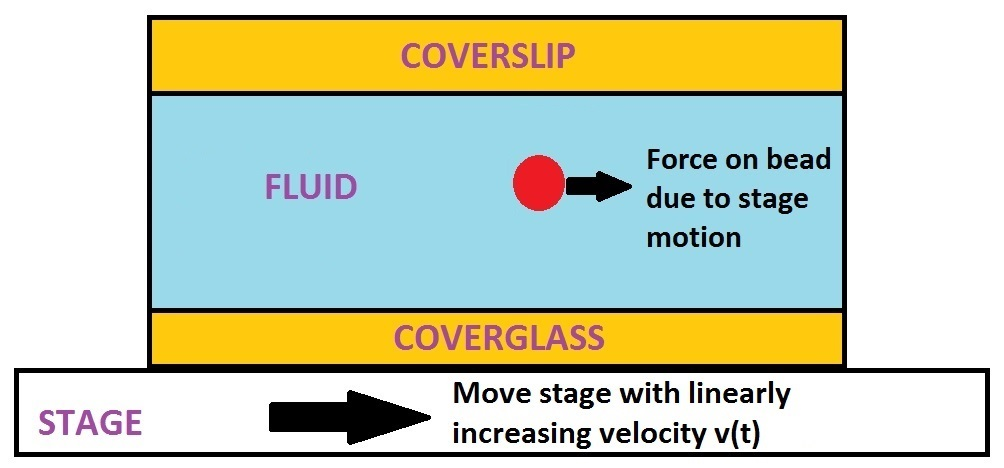
\includegraphics[height=6cm,width=11cm]{fig3.jpg}
 %   \caption{Applying step fitting to bead trace}
    \label{fig:graph3}
\end{figure}

\end{frame}

%%-----------------------------------------------------------------------
\begin{frame}{Work done in the Nature paper}

\begin{itemize}

\item Stage velocity $v$, viscous force on the bead $F = -\gamma v$
\item During erasure, magnitude of force increased linearly during time $\tau$ as $F(t)=\pm F_{max} . (t/\tau)$
\item Heat dissipated during tilt :
\begin{equation*}
Q= -\int_{0}^{\tau_{cycle}} F(t)\dot{x(t)}~dt=\pm \int_{0}^{\tau} F_{max}(t/\tau)\dot{x(t)}~dt
\end{equation*}
\item Velocity is calculated using the discretization
\begin{equation*}
\dot{x}(t+\Delta t/2) \approx [x(t+\Delta t)-x(t)]/\Delta t
\end{equation*}
\item For ideal quasi static erasure process $(\tau \rightarrow \infty)$ the dissipated heat equals Landauer's value

\end{itemize}


\end{frame}

%%-----------------------------------------------------------------------
\begin{frame}{Work done in the Nature paper}
\begin{figure}
    \centering
    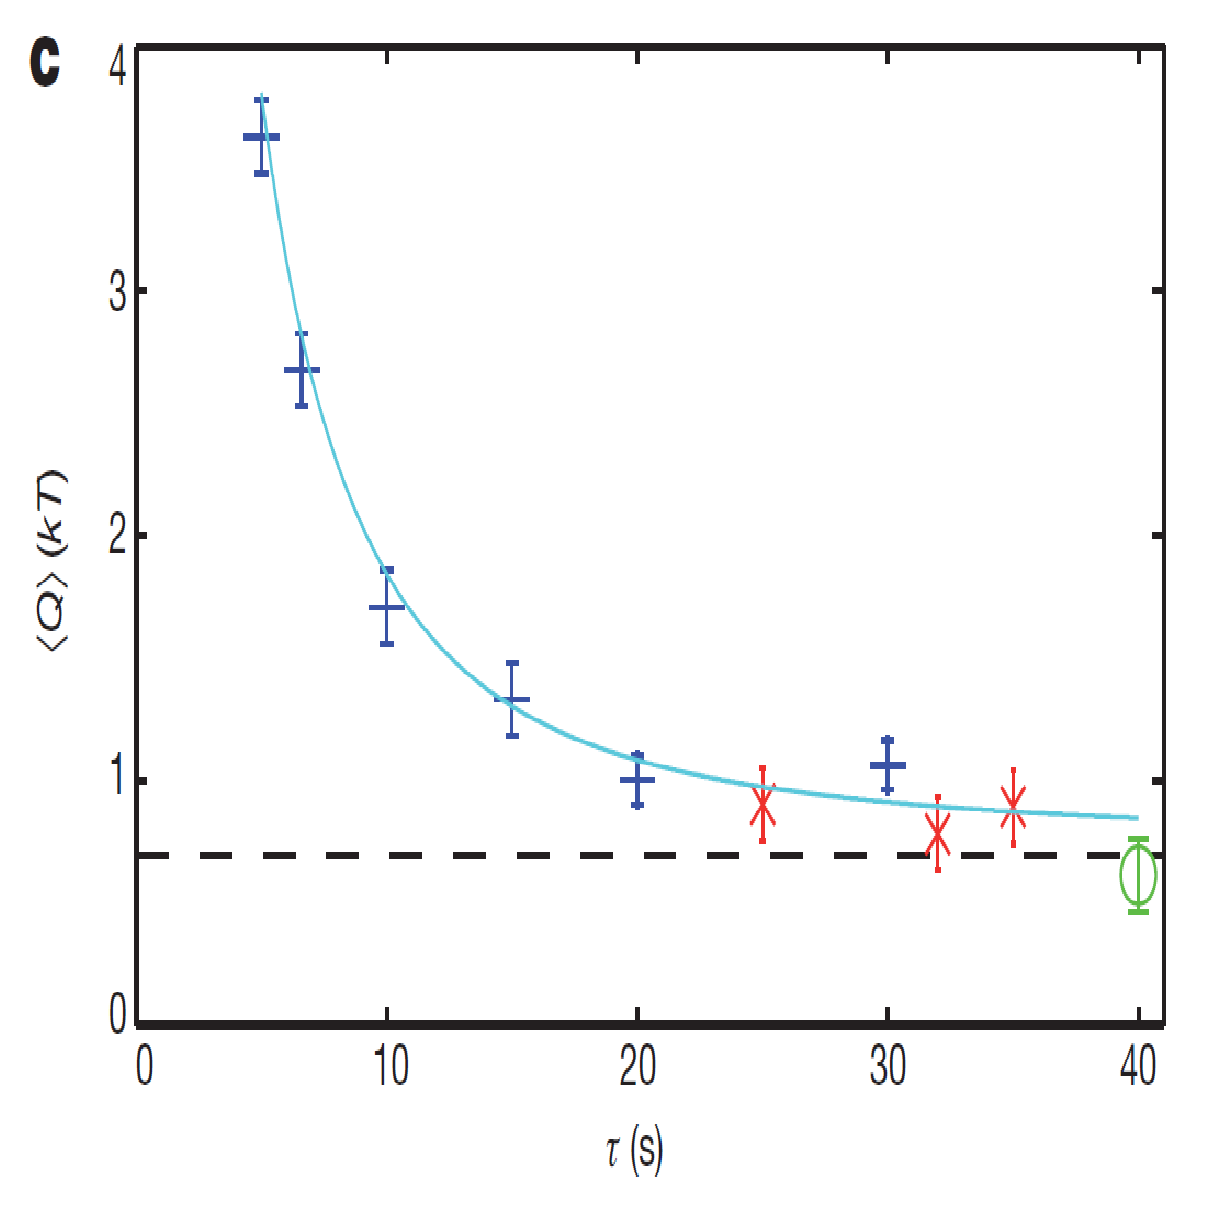
\includegraphics[height=5cm,width=11cm]{nature_landauer_fig4.eps}
 %   \caption{Applying step fitting to bead trace}
    \label{fig:graph4}
\end{figure}
plus sign r$\geq$ 90\% ; cross sign r$\geq$ 85\% ; circle sign  r$\geq$ 75\% where r is the success rate of the erasure protocol

\end{frame}
%%-----------------------------------------------------------------------
\subsection{Work done in EPL Paper}
\begin{frame}{Free energy using Jarzynski} 
When $r \rightarrow 1$ we have $<e^{-\beta W}> = 1/2$, then $\Delta F_{eff} \approx K_BT ln(2)$\\ All we need is the \textbf{work done} 
\begin{figure}
    \centering
    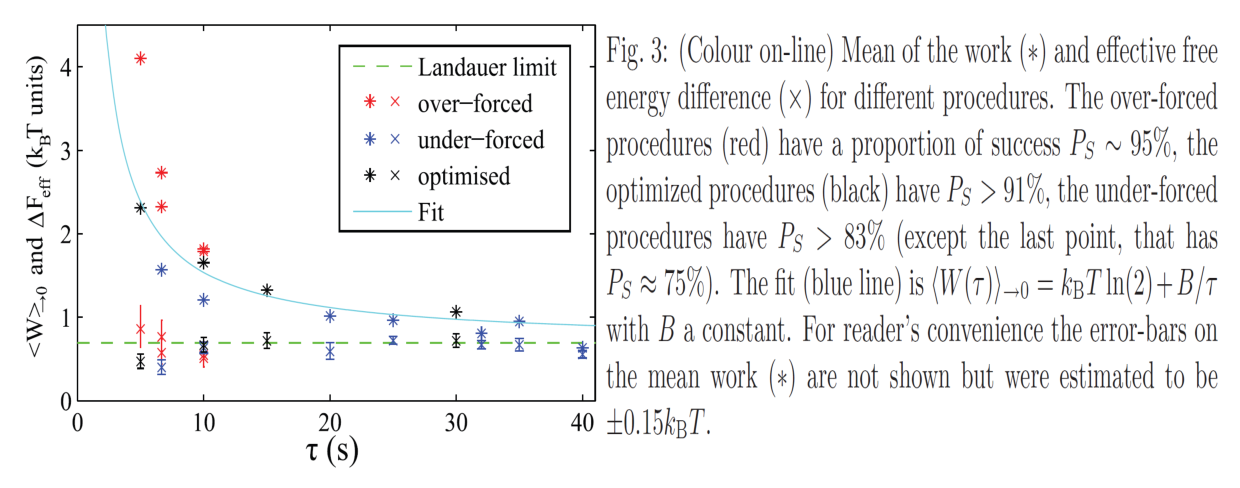
\includegraphics[height=5cm,width=11cm]{EPL_landauer_fig1.eps}
 %   \caption{Applying step fitting to bead trace}
    \label{fig:graph5}
\end{figure}

\end{frame}
%%-----------------------------------------------------------------------
\begin{frame}{Inference}
 
\begin{enumerate}

\item Work done calculated using $\int F .dx$ and averaged over several cycles should approach Landauer's limit
\item This work done is the \textbf{work done by external agency on the bead during the tilting of the wells}
\item The free energy difference calculated using Jarzynski equality converges to the limit independent of the value of the maximal force or procedure duration, so \textbf{from experimental viewpoint, Jarzynski equality enables us to perform experiments over a shorter duration}
\item \textit{Bottom-line} : We need to calculate work done in our case where tilting of wells is done by modulating the dwell times of the laser

\end{enumerate}

\end{frame}

%%-----------------------------------------------------------------------
\section{Preliminary calculations}
\subsection{Using drag force on the bead}
\begin{frame}{Using drag force on the bead}

\begin{itemize}

\item Force on bead due to viscous drag
\begin{equation*}
F_{drag}= -\gamma v = -6 \pi \eta R v
\end{equation*}
where $\eta$ is viscosity coefficient for water, R is bead radius and v is relative velocity between bead and medium
\item Work done = $\int_{0}^{\tau} F_{drag}dx = \int_{0}^{\tau} -(\gamma v) dx $
\item Two calculations are done :(1) Using unfiltered data and (2) Using filtered data with a 3-point MA filter$^{*}$
\item Question : How to decide $\tau ?$ We first considered total time, then time just around the transfer

\end{itemize}
${^*}$ \small{In the nature paper, they've processed the images to increase precision before using them}
\end{frame}

%%-----------------------------------------------------------------------
\begin{frame}{Using drag force on the bead}
Illustration on sample dataset
\begin{figure}
    \centering
    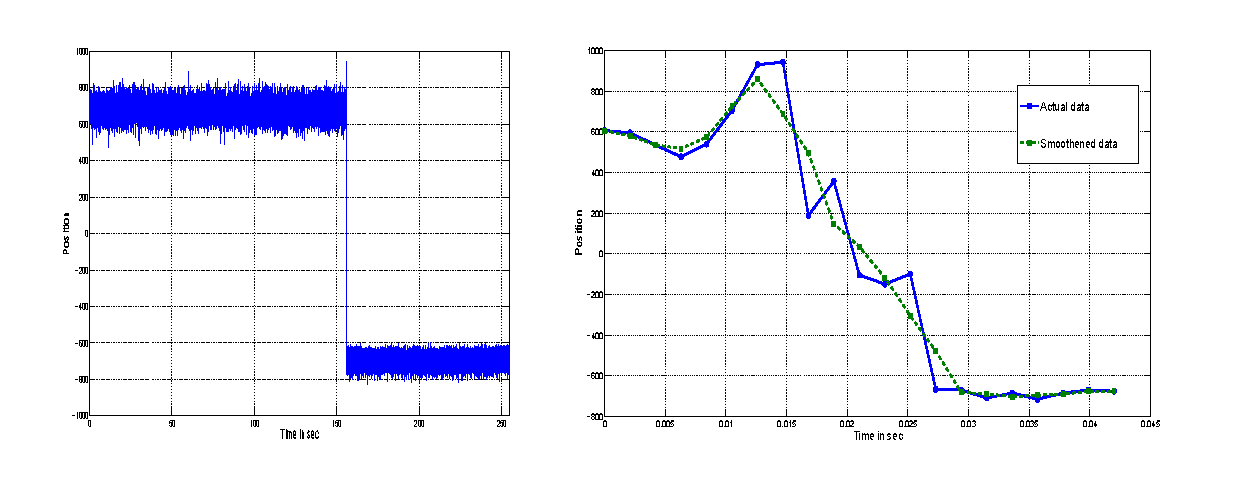
\includegraphics[height=5cm,width=11cm]{work_done_fig1.eps}
 %   \caption{Applying step fitting to bead trace}
    \label{fig:graph6}
\end{figure}

\end{frame}

%%-----------------------------------------------------------------------
\begin{frame}{Calculations-1}

$\eta=8.9 \times 10^{-4}$Pa.s for distilled water at $25^{\degree}$C\\
R = $500~nm$ and v = velocity of bead = $dx/dt$\\ $dt=0.002~sec~(500 H_z)$
\begin{table}
  \begin{tabular}{|c|c|c|c|c|}
    \hline
    \multirow{2}{*}{Dataset} &
      \multicolumn{2}{c|}{Total data ($K_BT$)} &
      \multicolumn{2}{c|}{Data around transfer ($K_BT$)} \\
      
    & Unfiltered & Filtered & Unfiltered & Filtered \\
    \hline
    1 & -111850 & -17956 & -2963.2 & -814.87  \\
    \hline
    2 & -204420 & -33144 & -1502 & -568.5  \\
    \hline
    3 & -169840 & -32520 & -12470 & -382.8  \\
    \hline
    4 & -265370 & -38830 & -689.3 & -251.93  \\
    \hline
    5 & -352990 & -70021 & -2351.3 & -600.51  \\
    \hline
    6 & -112830 & -19527 & -34864 & -590.9  \\
    \hline
    7 & -161950 & -29409 & -168937 & -579.40  \\
    \hline
  \end{tabular}
\end{table}
Clearly these are very high values !

\end{frame}
%%-----------------------------------------------------------------------
\begin{frame}{Analysis}

Issue I:
\begin{itemize}
\item The work done by drag force is dissipative
\item Motion of bead in either + or - direction will add to the dissipative work
\item Also, the more data points are considered, higher is be the work done calculated by this method
\item Bead position detected has some noisy component as well, which gets captured. It is clearly evident that filtering helps, but still not significantly enough
\end{itemize}


\end{frame}
%%-----------------------------------------------------------------------
\begin{frame}{Analysis}

Issue II:
\begin{itemize}
\item Coefficient of friction used by Nature Paper is $\gamma=1.89\times 10^{-10}$Ns/m for $2 \mu m$ diameter bead, which translates to $\eta=1.003\times 10^{-5}$Pa.s for our $1 \mu m$ bead
\item It is about \textbf{an order lower} than the $\eta$ we use, which is the standard coefficient for distilled water
\item To see its effect, I recalculated the work done using this lower $\eta$
\end{itemize}

\end{frame}
%%-----------------------------------------------------------------------
\begin{frame}{Calculations-2}

$\eta=1.003 \times 10^{-5}$Pa.s for distilled water at $25^{\degree}$C\\
R = $500~nm$ and v = velocity of bead = $dx/dt$
\begin{table}
  \begin{tabular}{|c|c|c|c|c|}
    \hline
    \multirow{2}{*}{Dataset} &
      \multicolumn{2}{c|}{Total data ($K_BT$)} &
      \multicolumn{2}{c|}{Data around transfer ($K_BT$)} \\
      
    & Unfiltered & Filtered & Unfiltered & Filtered \\
    \hline
    1 & -1253.5 & -201.22 & -33.2 & -9.131  \\
    \hline
    2 & -2290.8 & -371.42 & -16.83 & -6.37  \\
    \hline
    3 & -1903.3 & -364.42 & -13.97 & -4.289  \\
    \hline
    4 & -2301.5 & -435.13 & -7.724 & -2.823 \\
    \hline
    5 & -3955.7 & -784.68 & -26.416 & -6.729  \\
    \hline
    6 & -1264.4 & -218.82 & -39.06 & -6.622 \\
    \hline
    7 & -1814.8 & -329.56 & -18.93 & -6.4931  \\
    \hline
    
  \end{tabular}
\end{table}


\end{frame}

%%-----------------------------------------------------------------------
\begin{frame}{Analysis}

\begin{itemize}
\item Clearly, the lower value of $\eta$ has significant effect
\item When combined with filtering and using data around transfer, work done values seem practical

\end{itemize}
Several questions arise, which have been listed next

\end{frame}

%%-----------------------------------------------------------------------
\begin{frame}{Questions-1}

\begin{enumerate}
\item Is this approach using drag forces (dissipative work) correct ? In that case, it makes sense to \textbf{use only the data around transfer}.
\item Perhaps truncating the data around transfer might help even more ?$^*$
\item For calculating the drag force $F_{drag}$ we use $F_{drag}=-\gamma v$ where v is the velocity of bead. \\
According to Stokes law, v is the relative velocity between fluid and bead; so our assumption here is that the fluid is stationary(as we're not moving the stage). Is that correct ?


\end{enumerate}
 \tiny{Refer to rightmost column of table in the calculations-2 slide}

\end{frame}
%%-----------------------------------------------------------------------
\begin{frame}{Questions-2}

\begin{enumerate}
\item The coefficient of viscosity $\eta$ used in Nature paper (bidistilled water) is an order lower than ours (de-ionized water).\textit{Deionization produces a high purity water that is generally similar to distilled water}. Which to use ?
\item Filtering (3-point MA filter, the smallest one possible) has significant effect. How to decide which one to use ?
\item In our case where tilting is done due to different dwell times of blinking, what is the external parameter ? 
\item How do we calculate \textbf{work done on the bead} due to the variation of this external parameter ?

\end{enumerate}


\end{frame}
%%-----------------------------------------------------------------------

\subsection{Using total force on the bead}
\begin{frame}{Using total force on the bead}

\begin{itemize}

\item Total force on bead at given instant:
\begin{equation*}
F_{net}=m \ddot{x}= \frac{-\partial U}{\partial x}-\gamma v + noise
\end{equation*}
\item For given polystyrene bead with diameter $1\mu m$ bead density =$1.8189\times 10^{12}beads/gm$; so individual bead mass = $5.4978\times 10^{-16} kg$
\item Work done = $\int_{0}^{\tau} F_{net}dx$ where $\tau$ is \textit{time until just after the bead transfer} and $F_{net}=m \ddot{x}$
\item Work is calculated using unfiltered and MA filtered(window=3) bead position data
%\item Furthermore, contribution of drag force is calculated  without needing $\gamma$, by subtracting $\Delta U$ from $\int F_{net}dx$

\end{itemize}

\end{frame}

%%-----------------------------------------------------------------------
\begin{frame}{Using total force on the bead}
Illustration on sample dataset. Transfer at 156 s, data till $\tau=$161 s
\begin{figure}
    \centering
    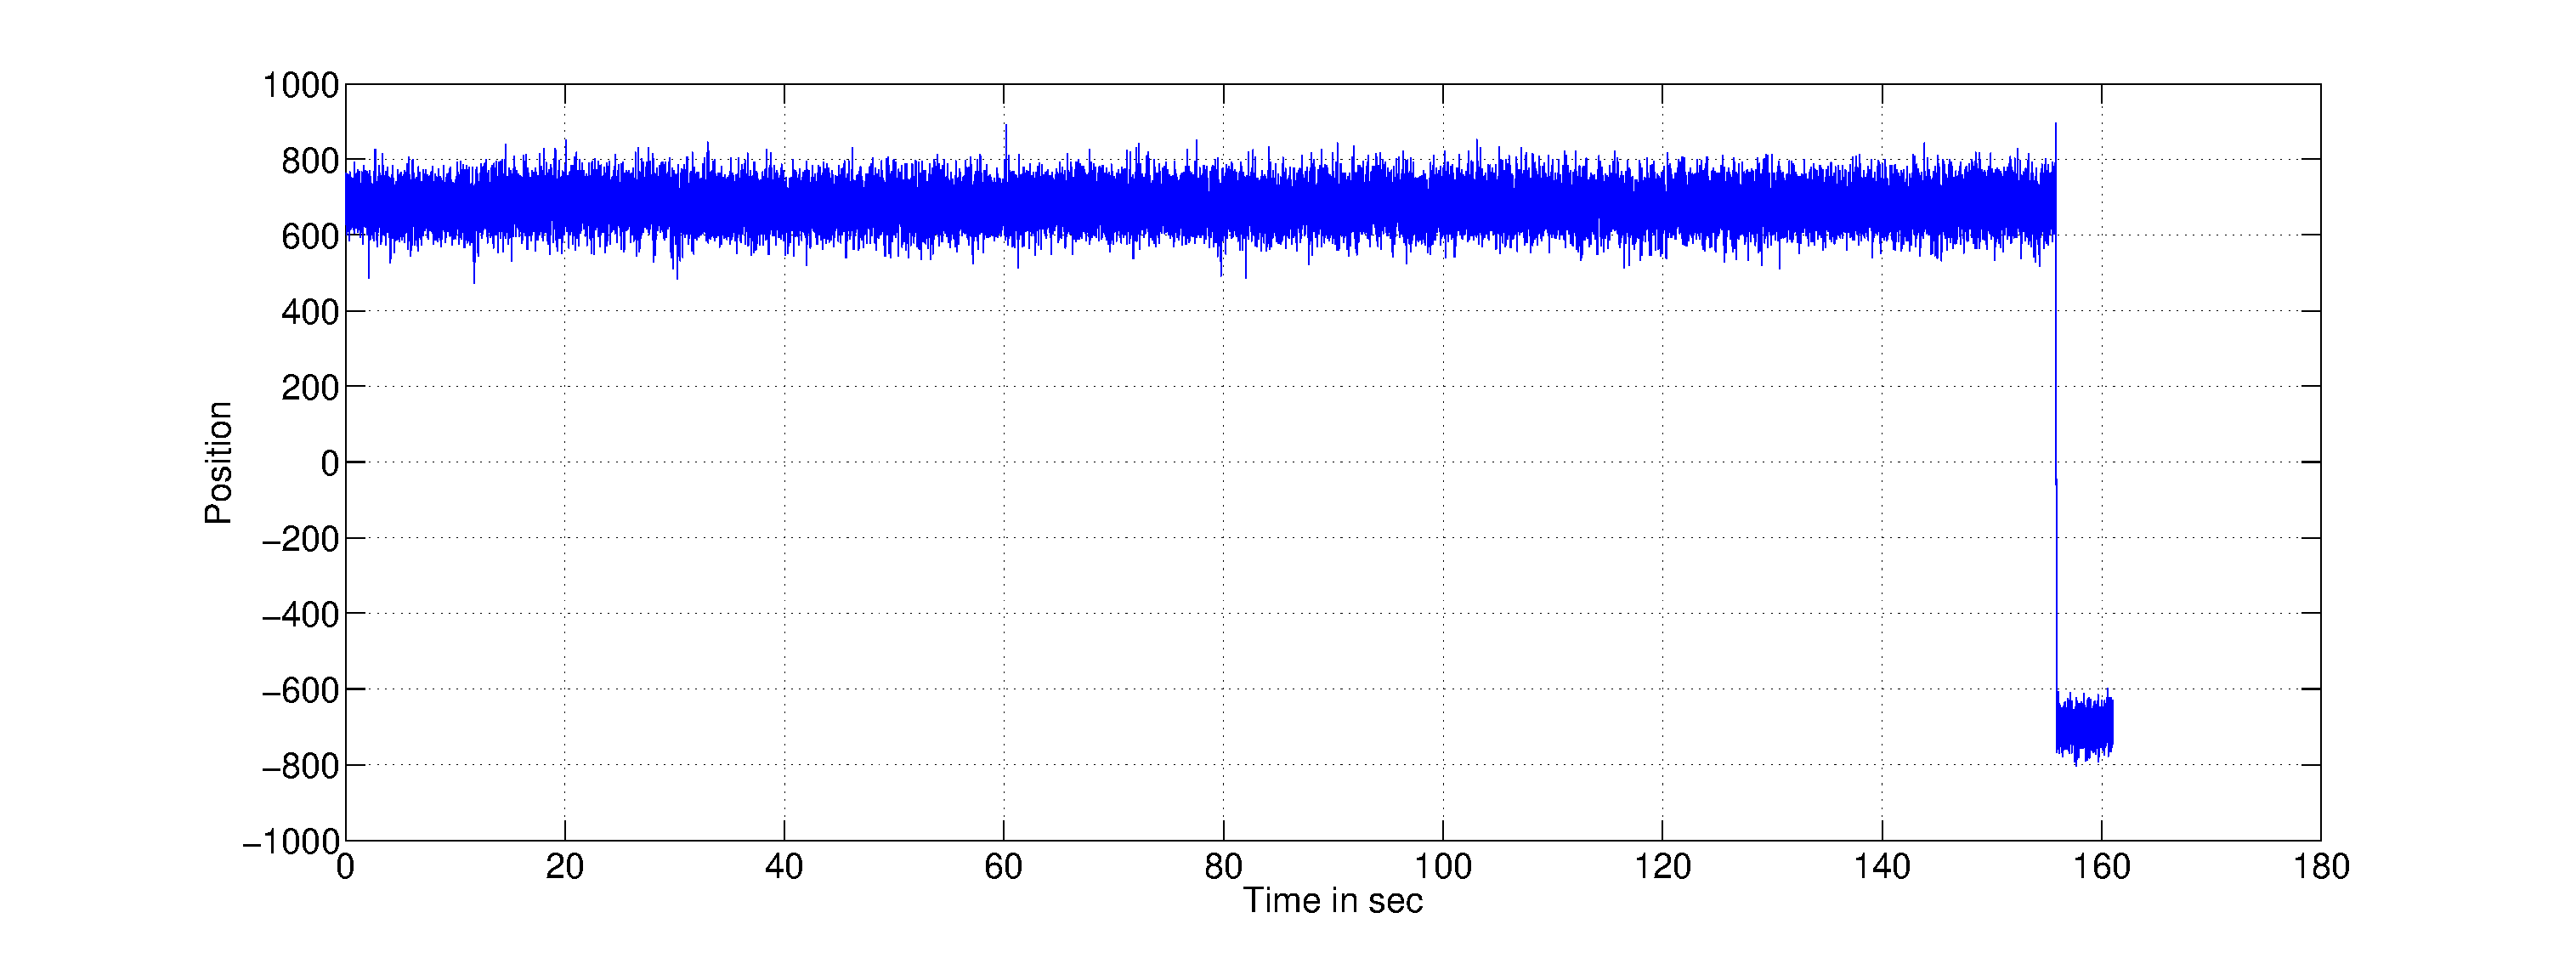
\includegraphics[height=5.5cm,width=11cm]{BddPos3_justafterTransfer.eps}
 %   \caption{Applying step fitting to bead trace}
    \label{fig:graph7}
\end{figure}

\end{frame}
%%-----------------------------------------------------------------------
\begin{frame}{Using total force $\rightarrow \tau$ just after transfer}
$\tau$ is till just after transfer
\begin{table}[h!]\scalebox{0.82}{
  \begin{tabular}{|c|c|c|c|c|c|}
    \hline
    \multirow{2}{*}{Dataset} &
      \multicolumn{2}{c|}{Work Done ($K_BT$)} &
      \multicolumn{2}{c|}{Well Potential ($K_BT$)} &
      \multicolumn{1}{c|}{$\Delta$ U } \\
%      \multirow{2}{*}{$\Delta U $ = $U_2 - U_1$ ($K_BT$)} \\
    & Unfiltered & Filtered & $U_2$(Left well) & $U_1$(Right well) & $U_2 - U_1$ ($K_BT$)\\
    \hline
    1 & -0.767 & -0.075 & 2.8 & 3.68 & -0.83  \\
    \hline
    2 & -3.21 & -0.289 &  3.2 & 3.55 & -0.35   \\
    \hline
    3 & -4.402 & -0.4246 & 3.5 & 3.25 & 0.25  \\
    \hline
    4 & -4.4706 & -0.4336 & 3.35 & 3.45 & -0.10  \\
    \hline
    5 & -7.1814 & -0.7003 & 3.55 & 3.35 & 0.20  \\
    \hline
    6 & -1.0911 & -0.1037 & 3.0 & 4.05 & -1.05  \\
    \hline
    7 & -2.855 & -0.269 & 3.25 & 3.65 & -0.40  \\
    \hline
  
    
  \end{tabular}}
\end{table}

\end{frame}

%%-----------------------------------------------------------------------
\begin{frame}{Using total force $\rightarrow \tau$ is entire dataset}
$\tau$ is entire dataset
\begin{table}[h!]\scalebox{0.82}{
  \begin{tabular}{|c|c|c|c|c|c|}
    \hline
    \multirow{2}{*}{Dataset} &
      \multicolumn{2}{c|}{Work Done ($K_BT$)} &
      \multicolumn{2}{c|}{Well Potential ($K_BT$)} &
      \multicolumn{1}{c|}{$\Delta$ U } \\
%      \multirow{2}{*}{$\Delta U $ = $U_2 - U_1$ ($K_BT$)} \\
    & Unfiltered & Filtered & $U_2$(Left well) & $U_1$(Right well) & $U_2 - U_1$ ($K_BT$)\\
    \hline
    1 & -1.3901 & -0.1303 & 2.8 & 3.68 & -0.83  \\
    \hline
    2 & -7.8841 & -0.6667 &  3.2 & 3.55 & -0.35   \\
    \hline
    3 & -7.015 & -0.6507 & 3.5 & 3.25 & 0.25  \\
    \hline
    4 & -8.5449 & -0.7862 & 3.35 & 3.45 & -0.10  \\
    \hline
    5 & -11.6882 & -1.091 & 3.55 & 3.35 & 0.20  \\
    \hline
    6 & -2.8291 & -0.2251 & 3.0 & 4.05 & -1.05  \\
    \hline
    7 & -6.034 & -0.5412 & 3.25 & 3.65 & -0.40  \\
    \hline
  
    
  \end{tabular}}
\end{table}

\end{frame}

%%-----------------------------------------------------------------------
\begin{frame}{Mean heat dissipated}
Using work done : Heat dissipated $Q=-\int_{0}^{\tau} Fdx$
\begin{center} 
\begin{tabular}{| c | c | c |} 
\hline  & Unfiltered & Filtered \\ 
\hline Data around transfer & 3.4253 & 0.3279  \\ 
\hline Total data & 6.4836 & 0.5845 \\ 
\hline 
\end{tabular} 
\end{center}

Using Jarzynski: $\Delta F_{eff}= -ln<e^{-\beta W}>$
\begin{center} 
\begin{tabular}{| c | c | c |} 
\hline  & Unfiltered & Filtered \\ 
\hline Data around transfer & 2.0265 & 0.3087  \\ 
\hline Total data & 3.1107 & 0.5386 \\ 
\hline 
\end{tabular} 
\end{center}


\end{frame}

%%-----------------------------------------------------------------------
\subsection{Calculating work due to drag force}
\begin{frame}{Work due to drag$\rightarrow \tau$ just after transfer}
$F_{net}=m \ddot{x}= \frac{-\partial U}{\partial x}-\gamma v$\\
$W_{net}= (U_2-U_1) + W_{drag}$ where $W_{drag}=\int_{0}^{\tau} F_{drag}dx=\int_{0}^{\tau} -(\gamma v) dx$\\
So $W_{drag}=W_{net}-\Delta U$
\begin{table}[h!]\scalebox{0.7}{
  \begin{tabular}{|c|c|c|c|c|c|c|c|}
    \hline
    \multirow{2}{*}{Dataset} &
      \multicolumn{2}{c|}{Work Done-Just after transfer ($K_BT$)} &
      \multicolumn{1}{c|}{$\Delta$ U } &
      \multicolumn{2}{c|}{$W_{drag}$ } \\
%     \multirow{2}{*}{$\Delta U $ = $U_2 - U_1$ ($K_BT$)} \\
    & Unfiltered & Filtered &  $U_2 - U_1$ ($K_BT$) &   Unfiltered & Filtered\\
    \hline
    1 & -0.767 & -0.075 &  -0.83 & & \\
    \hline
    2 & -3.21 & -0.289 &   -0.35 & & \\
    \hline
    3 & -4.402 & -0.4246 &  0.25 & &\\
    \hline
    4 & -4.4706 & -0.4336 &  -0.10 & &\\
    \hline
    5 & -7.1814 & -0.7003 &  0.20 & &\\
    \hline
    6 & -1.0911 & -0.1037 & -1.05 & &\\
    \hline
    7 & -2.855 & -0.269 &  -0.40 & &\\
    \hline
  
    
  \end{tabular}}
\end{table}

\end{frame}
%%-----------------------------------------------------------------------
\begin{frame}{Work due to drag$\rightarrow \tau$ is entire dataset}
$F_{net}=m \ddot{x}= \frac{-\partial U}{\partial x}-\gamma v$\\
$W_{net}= (U_2-U_1) + W_{drag}$ where $W_{drag}=\int_{0}^{\tau} F_{drag}dx=\int_{0}^{\tau} -(\gamma v) dx$\\
So $W_{drag}=W_{net}-\Delta U$
\begin{table}[h!]\scalebox{0.8}{
  \begin{tabular}{|c|c|c|c|c|c|c|c|}
    \hline
    \multirow{2}{*}{Dataset} &
      \multicolumn{2}{c|}{Work Done-Entire dataset ($K_BT$)} &
      \multicolumn{1}{c|}{$\Delta$ U } &
      \multicolumn{2}{c|}{$W_{drag}$ } \\
%      \multirow{2}{*}{$\Delta U $ = $U_2 - U_1$ ($K_BT$)} \\
    & Unfiltered & Filtered &  $U_2 - U_1$ ($K_BT$) &   Unfiltered & Filtered\\
    \hline
    1 & -1.3901 & -0.1303 &  -0.83 & & \\
    \hline
    2 & -7.8841 & -0.6667 &   -0.35 & & \\
    \hline
    3 & -7.015 & -0.6507 &  0.25 & &\\
    \hline
    4 &  -8.5449 & -0.7862 &  -0.10 & &\\
    \hline
    5 & -11.6882 & -1.091 &  0.20 & &\\
    \hline
    6 & -2.8291 & -0.2251 & -1.05 & &\\
    \hline
    7 & -6.034 & -0.5412 &  -0.40 & &\\
    \hline
  

    
  \end{tabular}}
\end{table}

\end{frame}
%%-----------------------------------------------------------------------
\begin{frame}


\end{frame}
%%-----------------------------------------------------------------------
\begin{frame}


\end{frame}


%%--------------------------------------------------------------------------------------------------------

%%--------------------------------------------------------------------------------------------------------








\end{document}


